\chapter{Introduction}\label{ch:intro}
\thispagestyle{empty}
\vspace*{\fill}
\epigraph{\emph{Genes are like the story, and DNA is the language that the story is written in}}
{--Sam Kean}

\clearpage
%%%%%%%%%%%%%%%%%%%%%%%%%%%%%%%%%%%%%%%%%%%%%%%%%%%%%%%%%%%%%%%%%%%%%%%%%%%%%%%%%%%%%
%%%%%%%%%%%%%%%%%%%%%%%%%%%%%%%%%%%%%%%%%%%%%%%%%%%%%%%%%%%%%%%%%%%%%%%%%%%%%%%%%%%%%
%%%%%%%%%%%%%%%%%%%%%%%%%%%%%%%%%%%%%%%%%%%%%%%%%%%%%%%%%%%%%%%%%%%%%%%%%%%%%%%%%%%%%
\section{Reading genome -- the book of life}
% * <hoangnguyen177@gmail.com> 2018-11-25T23:35:15.645Z:
% 
% maybe a grand-er opening ? 
% Like one of the greatest breakthrough in life science in 20th century is the ...
% history of genetic & central dogma?
The mission of decoding the genetic information of all organisms has been attracting great attention and effort from the research community over the past three decades. 
Although genomes are thought to contain nearly all the information necessary to create an organism, sequencing a genome is only the very first step towards understanding the development of an organism. 
Subsequent to genome sequencing and annotation there remains a huge amount of additional work to interpret the genome and understand how genes interact in pathways in a variety of contexts to sustain life. 
Nevertheless, the importance of the initial reading is indisputable as it would shape the details and output of any further analysis.
In fact, the competition of modern sequencing technologies have never been on hiatus, resulting in remarkably achievements in terms of both quality and quantity. 
However, unfortunately, we are still far away from having a flawless sequencer to date.

All genetic material of an organism is embraced in the term \emph{genome} mentioned earlier. Basically, the genome includes deoxyribonucleic acid (DNA) molecules -- the double helix polymers \cite{Watson1953} that virtually define a whole individual life form (except some viruses made by ribonucleic acid or RNA). 
A DNA molecule is a sequence of nucleotides, which is represented by 4 bases: adenine (A), cytosine (C), guanine (G), or thymine (T). The process of calling each and every single base of this sequence is known as \emph{DNA sequencing}. Sequencing an entire organism's genome is termed Whole Genome Sequencing (WGS). 
Innovation in sequencing technology has enabled WGS for a large variety of species with increasing genome sizes and complexity  over time, such as \emph{Haemophilus influenzae} bacterium \cite{Fleischmann1995}, \emph{Saccharomyces cerevisiae} \cite{Goffeau1996}, \emph{Caenorhabditis elegans} \cite{Sequencing1998} and \emph{Mus musculus} (mouse) \cite{Chinwalla2002}. Ultimately, the completion of the Human Genome Project \cite*{International2004} marked the beginning of the genomic era in which rapidly developing technology would make WGS much more efficient and affordable.
The cost of sequencing has been dropped drastically over time to the point that scientists are now planning for the Earth BioGenome Project, which plans to sequence 1.5 million different species across multiple continents\cite{Lewin2018earth}.

%%%%%%%%%%%%%%%%%%%%%%%%%%%%%%%%%%%%%%%%%%%%%%%%%%%%%%%%%%%%%%%%%%%%%%%%%%%%%%%%%%%%%
%%%%%%%%%%%%%%%%%%%%%%%%%%%%%%%%%%%%%%%%%%%%%%%%%%%%%%%%%%%%%%%%%%%%%%%%%%%%%%%%%%%%%
\subsection{DNA sequencing technology}

\begin{figure}[ht!]
\centering
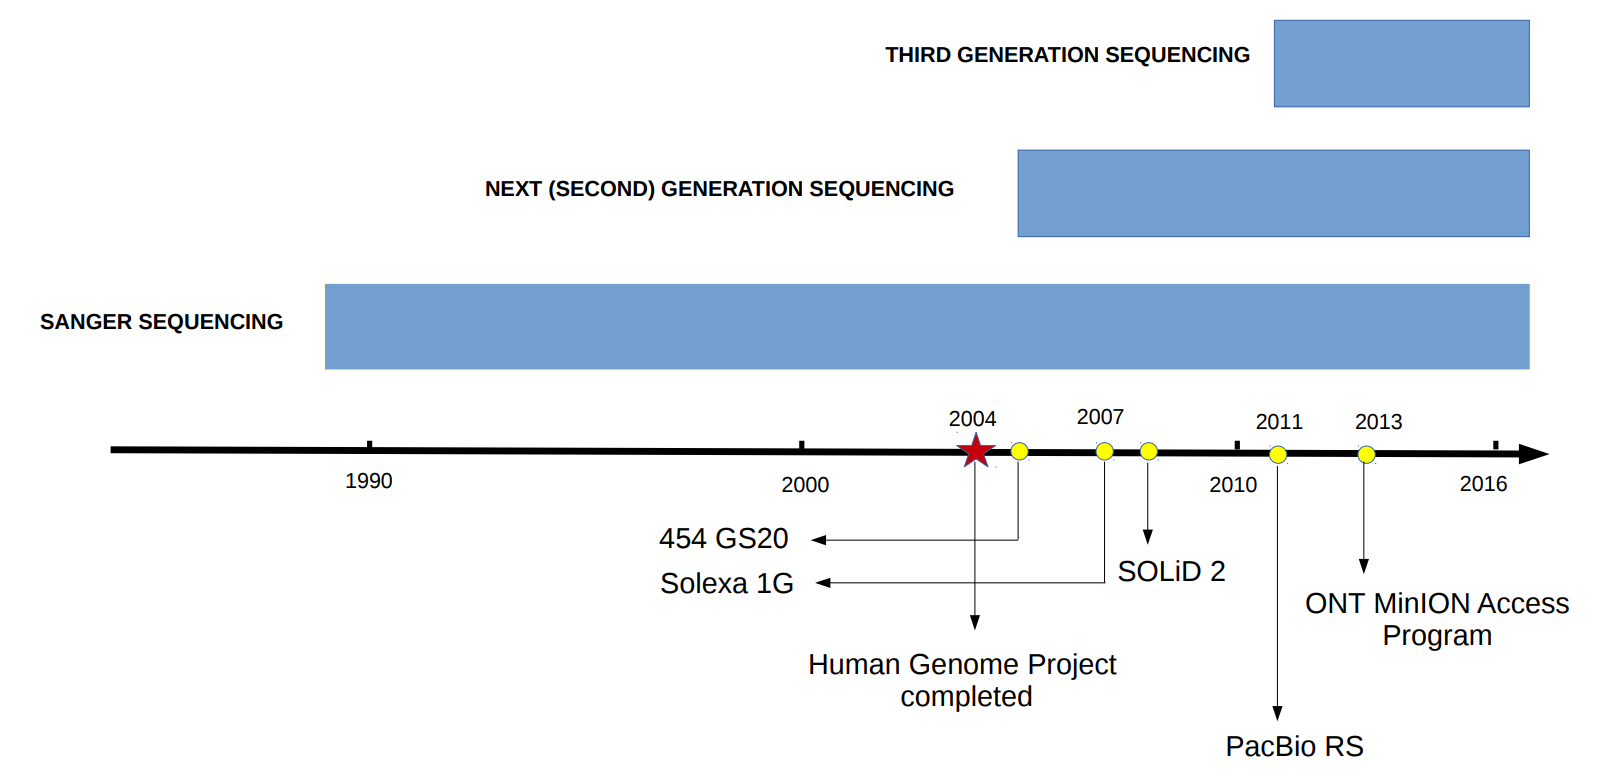
\includegraphics[width=.9\textwidth]{images/timeline.png}
\caption{Prominent sequencing platforms in the era of genomics.}
\label{Fig:nanopore}
\end{figure}
The first practical sequencing technology was invented by Frederick Sanger and colleagues \cite{Sanger1977} and as the consequence, had been named after its founder. 
Sanger sequencing, can be considered as the \emph{First generation sequencing}, employs the mechanism of selectively terminating the chain elongation by dideoxy nucleotide, which is a nucleotide analogue which lacks a 3`-hydroxyl group needed for the next incorporation and extension.
Improved Sanger platforms nowadays can output reads up to around $1$Kbp with high accuracy (99.9\%) but the yields and cost are still unreasonable compared with other methods.
In fact, Sanger sequencing contributed vastly at the beginning of the sequencing era but became supplanted later by \emph{Second-Generation Sequencing} (SGS) machines (previously known as Next-Generation Sequencing) which are of much larger scale and higher throughput in term of data acquired. For that reason, it is restricted in use today, and used largely only for validation or in combination with other deep-sequencing methods \cite{Freeman2009}.
SGS platforms, on the other hand, can output a large amount of DNA sequence with length up to $1$Kbp in form of single, mate-paired or paired-end reads on demand, for a large ranges of studies.
Prominent sequencing technologies include pyrosequencing \cite{Ronaghi1996,Ronaghi1998} 
(Roche 454), ion torrent(ThermoFisher), SOLiD sequencing (Applied Biosystems) and sequencing by synthesis (Illumina/Solexa).

\begin{table}[ht!]
\centering
\caption[Comparison of DNA sequencing methods in general]{Comparison of DNA sequencing methods in general. Each method may have several platforms with varied configurations for different usage. More details in \cite{Lee2013common,Mardis2017dna}.} 
\label{tab:sequencing}
\begin{tabular}{llcccc}
\hline
\toprule
\multirow{2}{*}{\textbf{Gen.}} & \multirow{2}{*}{\textbf{Sequencing methods}}& \textbf{Read length} & \textbf{Accuracy} & \textbf{Reads}  & \textbf{Time} \\
& & \textbf{(bp)} & \textbf{(\%)} & \textbf{per run} & \textbf{per run} \\ 
\hline
\rowcolor{Gray}
 \cellcolor{white} & Chain termination &  &  &  & \\
\rowcolor{Gray}
 \cellcolor{white} \multirow{-2}{*}{$1^{st}$} & (Sanger sequencing) &\multirow{-2}{*}{$400-900$} & \multirow{-2}{*}{$99.9$} & \multirow{-2}{*}{N/A} & \multirow{-2}{*}{$0.3-3$ hours} \\
\hline
 & Pyrosequencing (454) & $700$ & $99.9$ & $1$ million & $24$ hours\\
\rowcolor{Gray}
 \cellcolor{white} & Sequencing by synthesis &  &  & up to & \\
\rowcolor{Gray}
 \cellcolor{white} & (Illumina/Solexa) & \multirow{-2}{*}{up to $300$} & \multirow{-2}{*}{$>99$} &  $3$ billions & \multirow{-2}{*}{$<1-14$ days}\\
& Sequencing by ligation & \multirow{2}{*}{$75+35$} & \multirow{2}{*}{99.9} & up to & \multirow{2}{*}{$1-2$ weeks} \\
& (SOLiD sequencing) & & & $2.8$ billions & \\
\rowcolor{Gray}
 \cellcolor{white} \multirow{-6}{*}{$2^{nd}$} & Ion semiconductor & $200$ & $98$ & $5$ millions & $2$ hours\\
\hline
 & Single molecule,  & $3000$ & \multirow{2}{*}{$85$} & \multirow{2}{*}{$\approx 50$K} & \multirow{2}{*}{$2$ hours} \\
 & real-time sequencing &  on average & & & \\
\rowcolor{Gray}
 \cellcolor{white} &  & extremely &  & $\approx 150$K & $<48$ hours\\
\rowcolor{Gray}
 \cellcolor{white}\multirow{-3}{*}{$3^{rd}$} & \multirow{-2}{*}{Nanopore sequencing} & long & \multirow{-2}{*}{$85-96$} & per flow cell & (real-time output) \\
\hline
\end{tabular}
\end{table}  

After years of innovation, Illumina is currently leading the sequencing market. This giant company reportedly has much larger revenues compared to other competitors~\cite{Philippidis2018top}
%estimated as \$$2.752$ billions in 2017 
and its equipment is ubiquitous amongst genomics labs worldwide. 
In fact, the sequencing productivity, quality and deployment cost-effectiveness have been enhanced significantly with the introduction of new platforms such as MiniSeq, MiSeq series, NextSeq, HiSeq and HiSeq X and Novaseq series. These sequencers provide high-fidelity paired-end reads of length 100-300bp each.  In consequence, bacterial DNA sequencing is typically done at average sequencing depth of more than 100-folds.
In other words, each of every bases in the whole genome would be covered by around 100 reads using such platforms.
In this thesis, data from Illumina MiSeq or HiSeq were used as input for the assembly algorithms. 

The race for better sequencing technology is still going on rapidly and intensively, illustrated by the emergence of so-called \emph{Third generation} or long-read sequencing technology \cite{Munroe2010third,Bleidorn2016third} with two major representatives \IE{} Pacific Biosciences of California, Inc. (PacBio) and Oxford Nanopore Technologies Limited (ONT). 
As indicated by the name, the defining feature of this category is the ability to measure in real-time the signals of every single molecule and output significantly longer reads than the previous generation sequencers. 
Table \ref{tab:sequencing} presents the performances of above-mentioned sequencing platforms in term of read length, yield, accuracy and running time.

At the time this thesis being written, Illumina has come to an agreement to acquire PacBio for approximately \$$1.2$ billions in an attempt to expand its DNA sequencing capacity. At the same time,  ONT is continuing to grow into a essential player in the field of genome sequencing with remarkable success stories.
The next section will briefly shed light into TGS focusing on the latter technology.

%%%%%%%%%%%%%%%%%%%%%%%%%%%%%%%%%%%%%%%%%%%%%%%%%%%%%%%%%%%%%%%%%%%%%%%%%%%%%%%%%%%%%
\subsection{Third-generation sequencing technology}
\paragraph{Single molecule, real-time (SMRT) sequencing}
The first long-read sequencer available on market was the PacBio RS from Pacific Biosciences of California, Inc. in 2011. 

\begin{figure}[ht!]
\centering
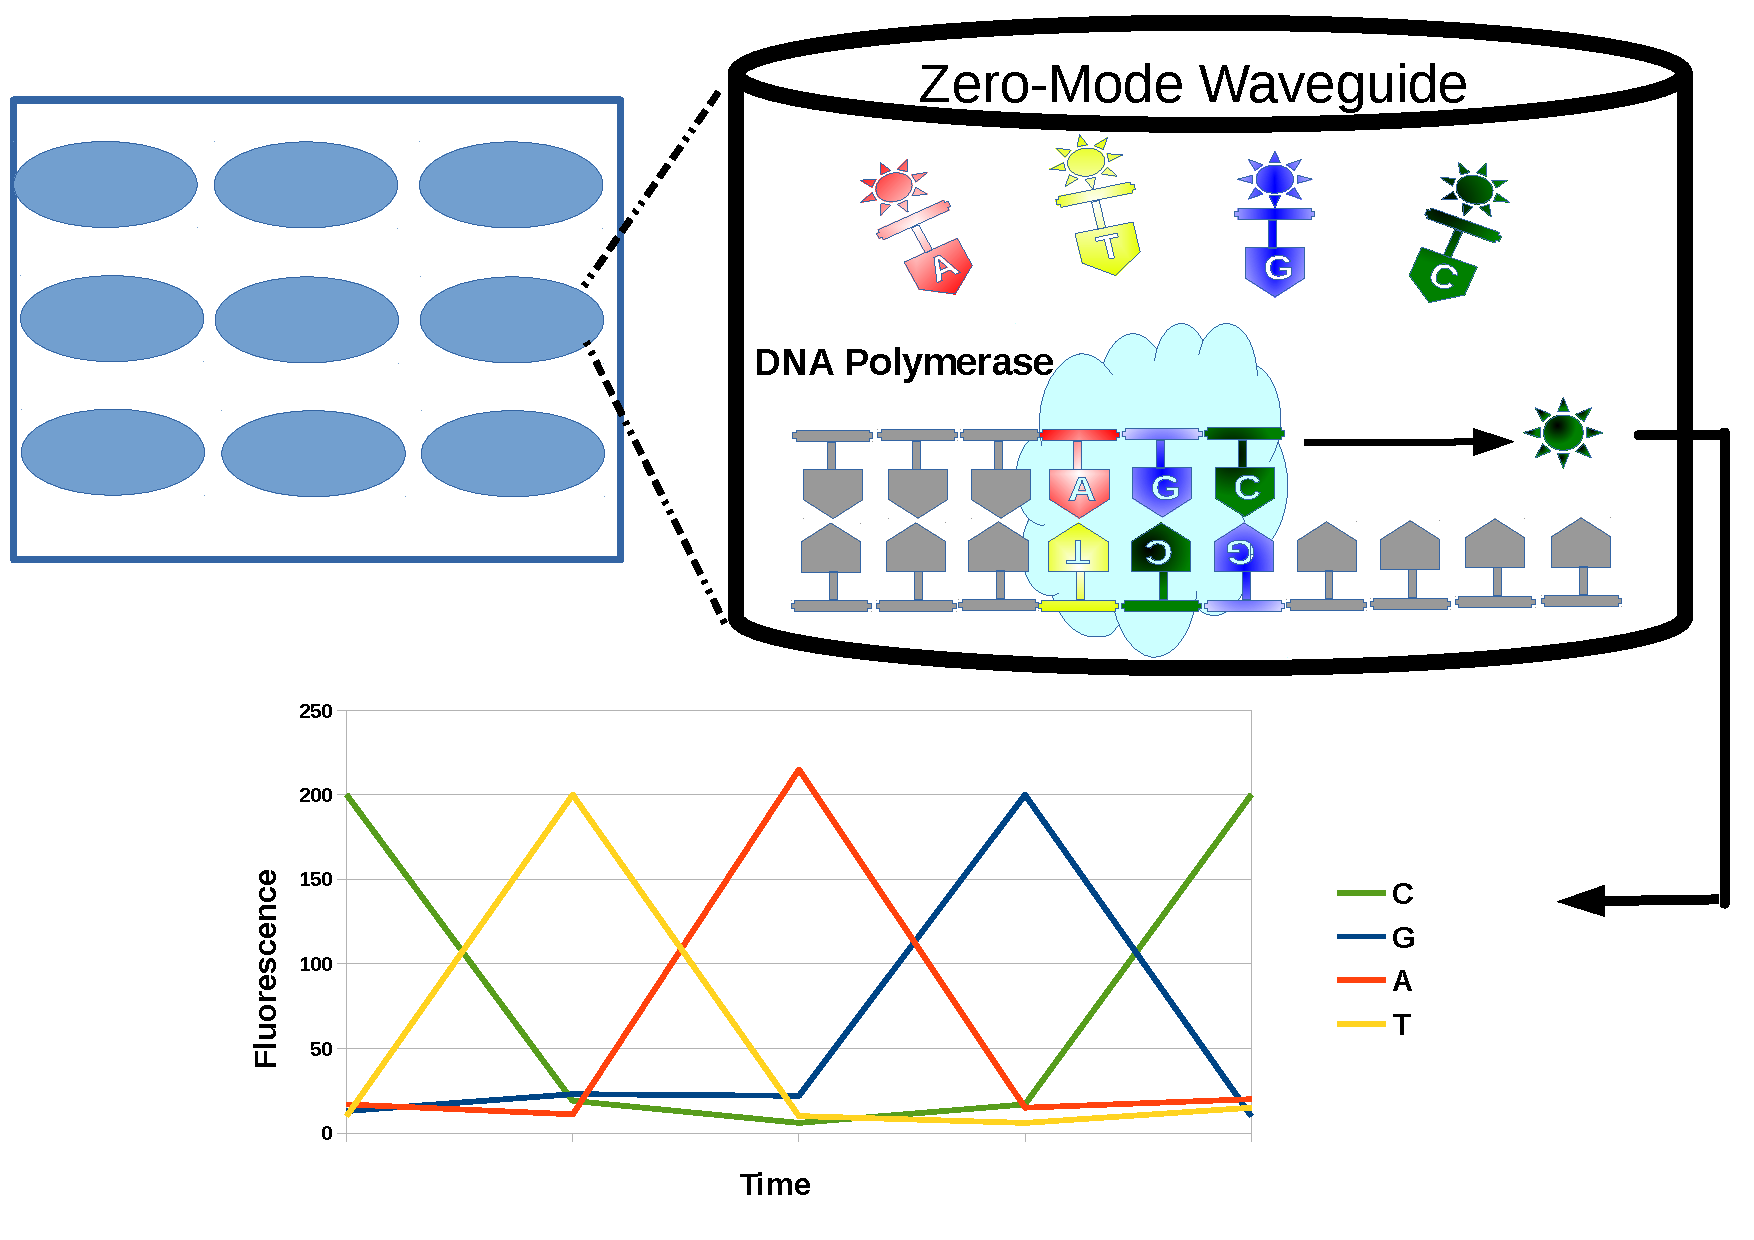
\includegraphics[width=.8\textwidth]{images/pacbio.pdf}
\caption{Mechanism of SMRT sequencing with Zero-Mode Waveguides.}
\label{F:pacbio}
\end{figure}

The SMRT technology takes advantage of \emph{zero-mode} waveguides (ZMW) to detect the activity of DNA polymerase incorporating a single nucleotide at a time \cite{Rhoads2015}. 
A ZMW structure consists of a circular hole in sub-wavelength scale ($20\times10^{-21}$ litre volume) in a metal film \cite{Korlach2008selective}. A complex of DNA polymerase and a single stranded template DNA molecule is immobilized at the bottom of the chamber surrounded by fluorescent dyed bases, as shown in Figure \ref{F:pacbio}. The DNA synthesis activity cleaves off the dyed tag of each incorporated base which can be detected optically in real-time within this smallest available microscopy structure \cite{Levene2003zero}. A SMRT cell can harbor thousands (RS platform) to hundred thousands (RS II) or even millions of ZMWs (Sequel, 8M chip) to facilitate parallelization and thus improve the throughput per cell. 

In fact, both the read length and accuracy of the instrument have been continuing to increase significantly. The average accuracy per read has increased from about 82\% in the first release to 87\% \cite{Eid2009,Koren2013} whilst the maximum read length has reached over $50$Kbp in recent runs \cite{Berlin2015}. 
As the consequence, PacBio DNA reads have gone from only being used in hybrid assembly which required high-fidelity complementary reads \cite{KorenSW2012, Ribeiro2012}, to now being able to generate finished \emph{de novo} bacterial genomes on its own \cite{Koren2013}.

\paragraph{Oxford Nanopore sequencing} 
In late 2013, ONT released the first nanopore sequencer, the \emph{MinION}, in the \emph{MinION Access Program} (MAP).
MAP was offering opportunity to researchers worldwide to have access on the third-generation reads. 
Of the particular advantages using this device is its greater portability and flexibility.

\begin{figure}[h]
\centering
\subfloat[Sequencing with MinION\label{fig:minion}]{
	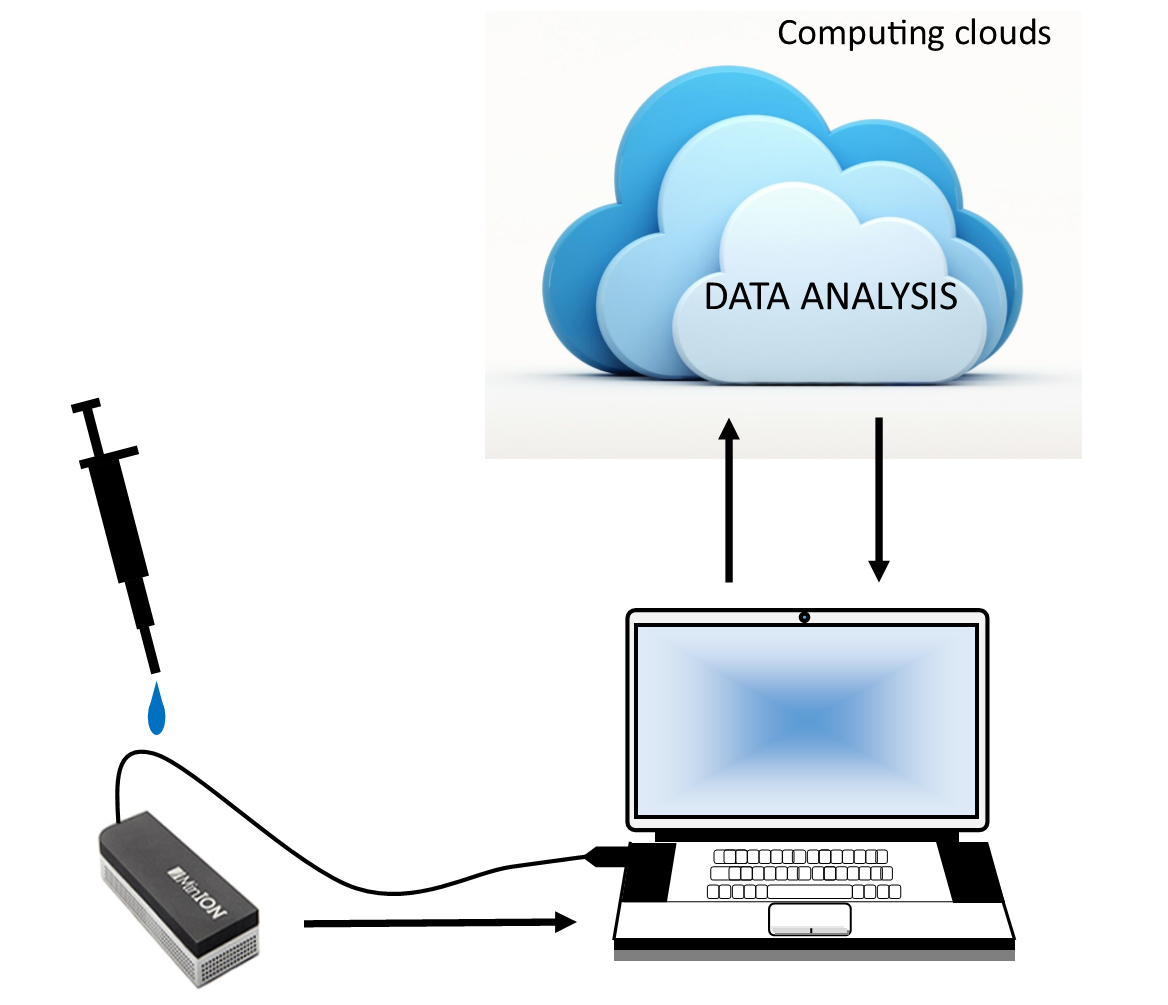
\includegraphics[width=.55\textwidth]{images/mnanopore.png}
}
\hfill
\subfloat[Inside the pore\label{fig:pore}]{
	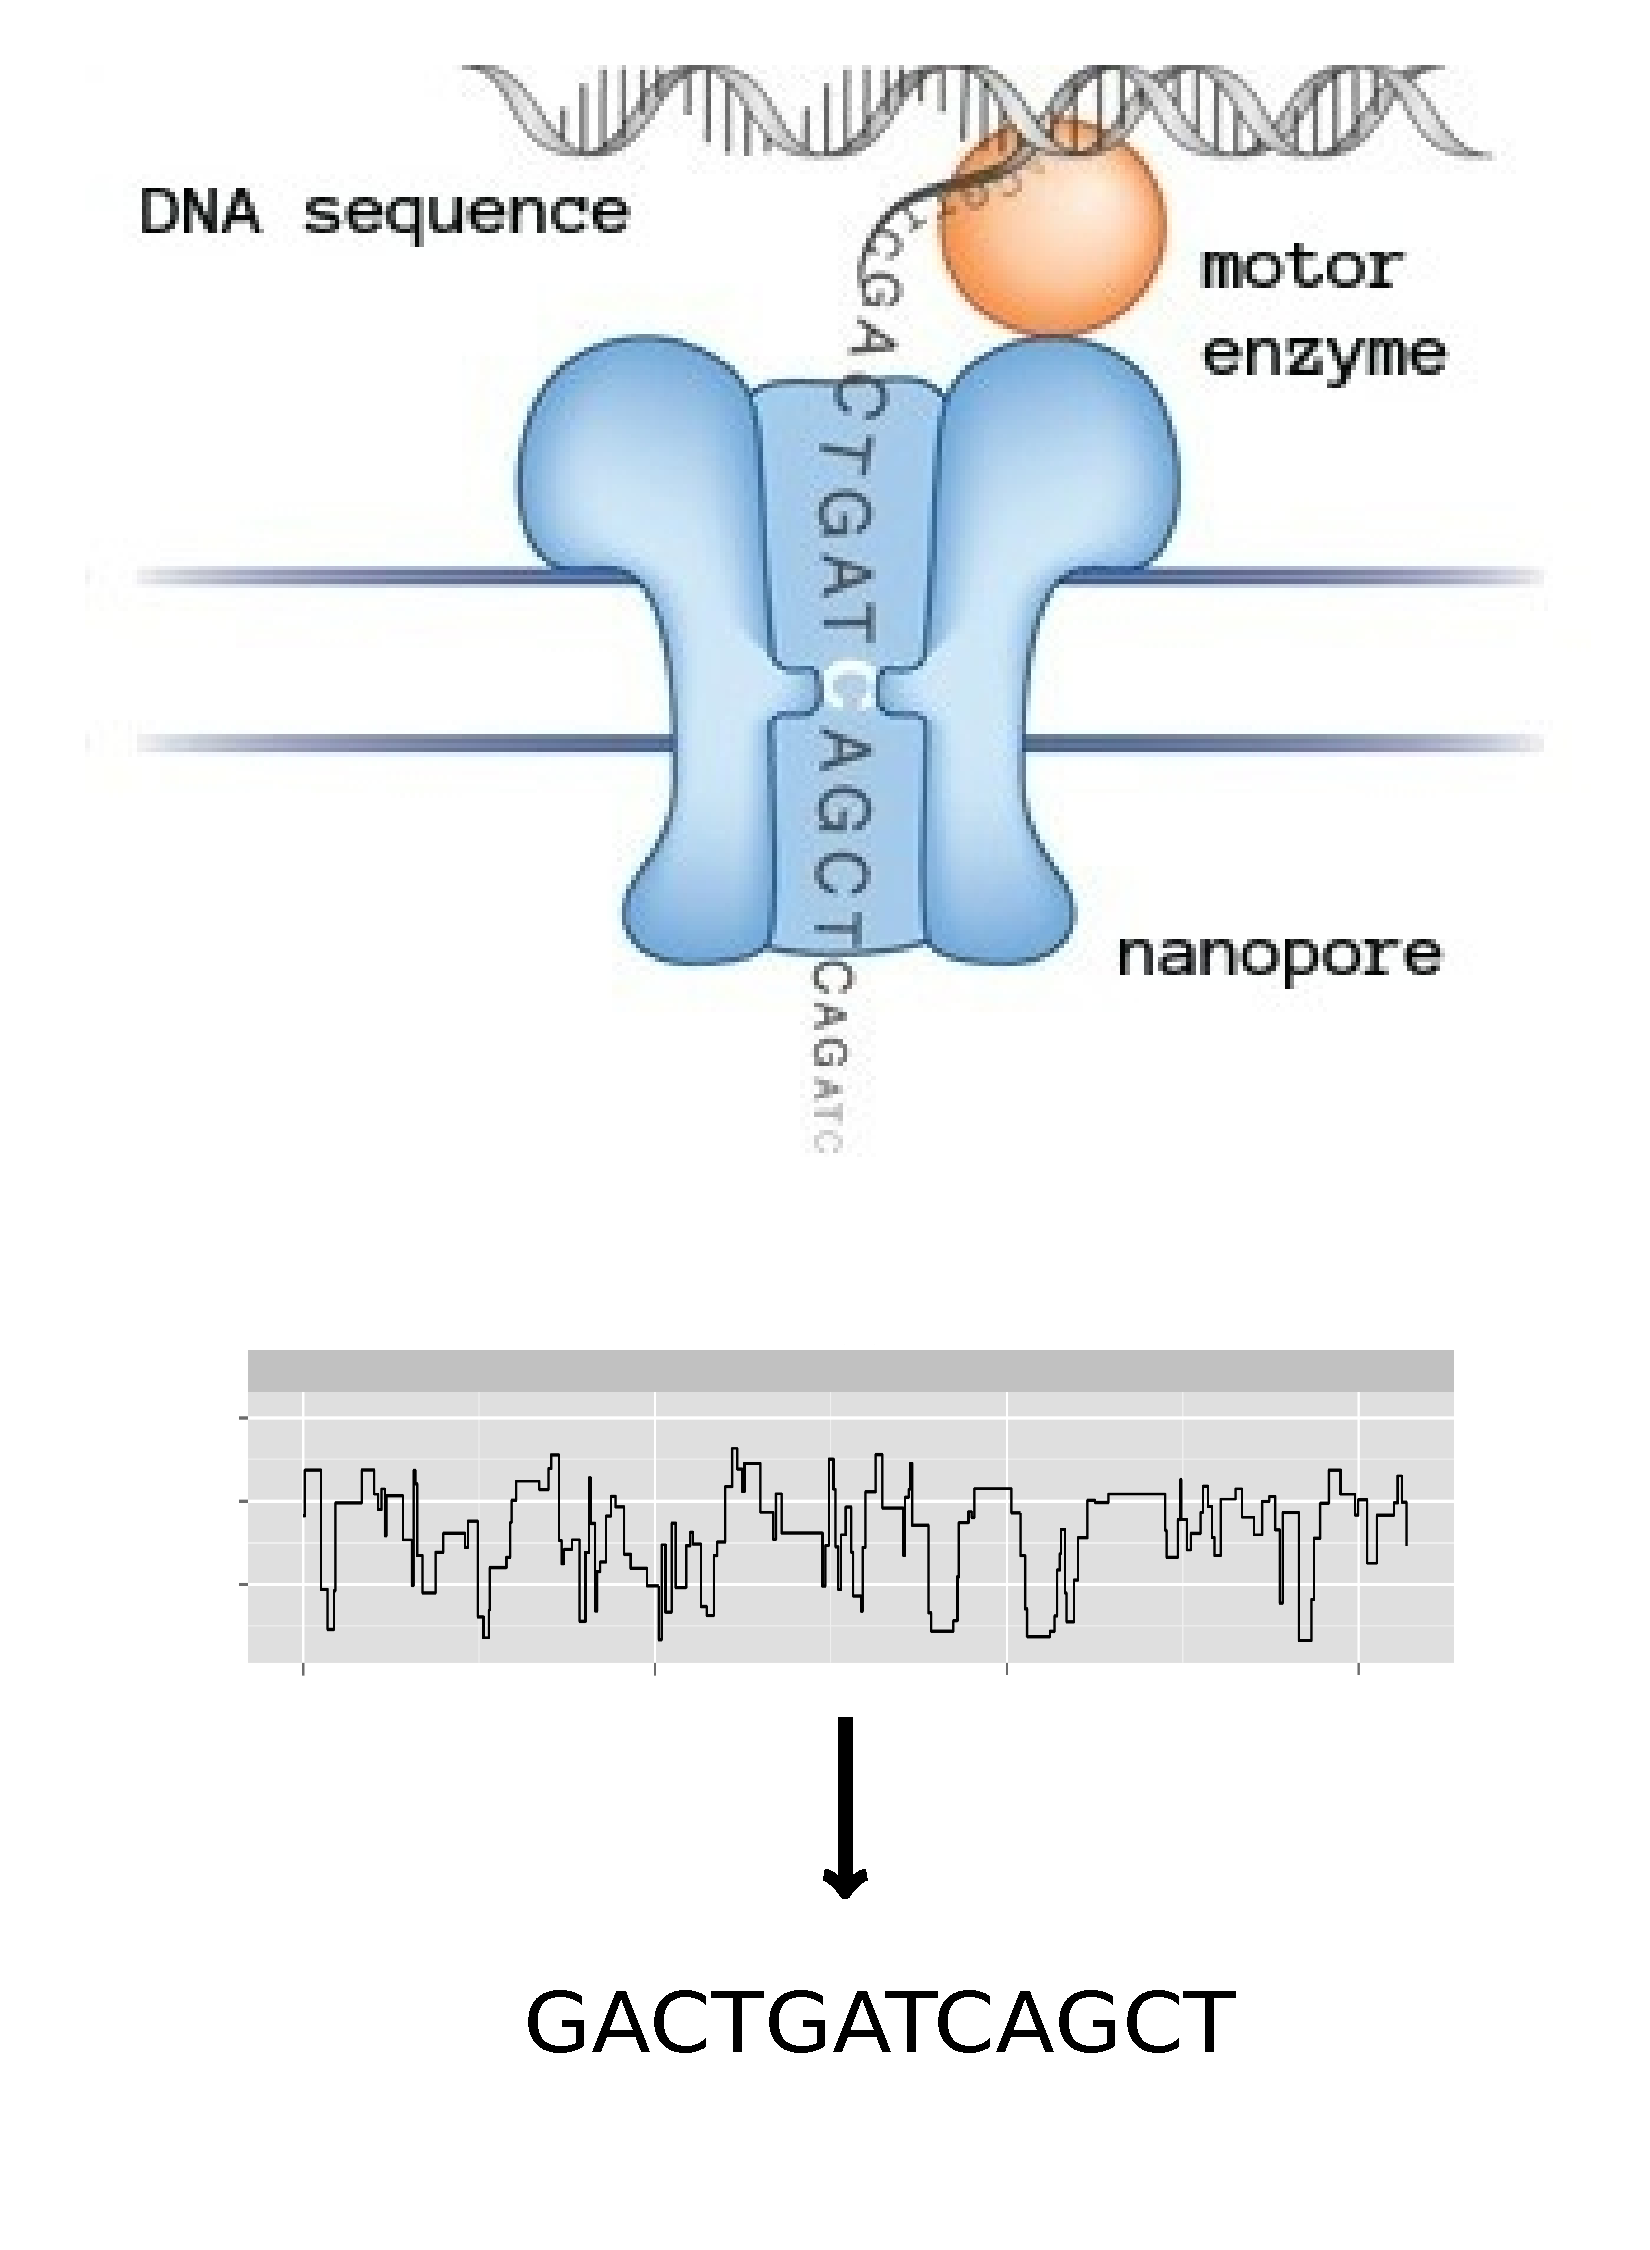
\includegraphics[width=.35\textwidth]{images/pore.pdf}
}
\caption[Illustration of nanopore sequencing with MinION]{Illustration of nanopore sequencing with MinION. (a) General setup for MinION sequencing. (b) Nanopore sequencing mechanism at molecular level.}
\label{F:nnp_run}
\end{figure}

Figure \ref{fig:minion} presents a general workflow of a sequencing run using MinION.
After DNA extraction, the very first step -- sample and library preparation, is straightforward but can also be varied for different experimental aims, such as maximizing yield, accuracy or read-length; as well as different experimental conditions, such as amount and quality of starting DNA.  
The purpose of library preparation is to bring necessary adapters and/or chemistry to the input mixture prior to the sequencing. 
ONT provides a variety of sequencing kits for different purposes.  For example, using the Rapid Sequencing Kit is simple and quick (10 minutes in theory) that would fit experiments with critical time and resource condition \EG{} remote locations. On the other hand, the Ligation Sequencing Kit family is more time-consuming  (about an hour) but gives better control over read length.
Other than these, ONT offers expansion packs for diverse project scenarios such as Barcoding kits for multiplexed sequencing or Low input kits for sequencing as little as $10$ng of DNA molecules.
In addition, if better quality is desired, users could, in the early stages, consider using a 2D kit (which would sequence both DNA strands in a single read), which has been replaced with an updated 1D$^2$ protocol (which with high probability sequences the second strand in the same pore immediately after sequencing the first strand, but as a separate read). 
After loading the prepared mixture to the device, the sequencing and base-calling phases could be employed automatically and \emph{in situ} thanks to the built-in services. In combination with a MinION, it is only required to have an internet-connected laptop with proper software installed to run the experiment, making it possible to establish sequencing-on-the-field where access to lab equipment is limited.

Figure \ref{fig:pore} illustrates the sequencing mechanism in more details.
In fact, the general mechanism of an artificial nanopore has been proposed \cite{Kasianowicz1996,Church1998} long before being applied as a real DNA sequencing technique by Hagan Banley and ONT \cite{Clarke2009}. 
In which, the unwound molecules are threaded through a nano-scaled pore on an electrically charged membrane protein known as \emph{the nanopore}. 
In the whole process, the velocity of the molecule translocating through the pore is controlled by a motor enzyme.
The rationale of this technology is that the shift of nucleotide sequence inside of a pore leads to the variation in its electrical resistance, resulting in a change in the current signal which is recorded as squiggles by time. These squiggle signals are feasibly translated back to the format of strings of nucleotide identities.
Indeed, a Hidden Markov Model (HMM) \cite{Baum1966,Baum1970} in the older version of Albacore, or Recurrent Neural Network (RNN) deep learning algorithm in later versions of Albacore, Chiron~\cite{teng2018chiron}, Guppy are used to study the transition and predict the sequence of DNA that most likely would generate these signals. 
Due to the  unavoidable noises of the measures in such tiny scale, a certain innate level of error may be expected from the base callers, although ONT has proposed using a variety of different types of pores simultaneously in order to generate independent error profiles. 

The nanopores are packed into a \emph{flow cell}, which is the consumable of this technology. Start-up cost of operating MinION is virtually zero, as users only have to pay for running costs, making it suitable for any project scale.  
The chemistry and computational features are likewise updated continuously to help reduce the noises from output. Recently, R10 flow cell is made available for higher signal accuracy, together with the newest base-calling algorithm from Guppy flip-flop pipeline that supports GPU for heavy computational deep-learning tasks, it has shown positive progress of this sequencing technology to tackle errors. When the demand of resources optimization is concerned, \emph{flongle} (single-use flow cell) can be used for small genomes. On the other hand, washing kits can be applied to reactivate pores from an interrupted flow cell, making it ready for another run.  

Furthermore, GridION and ProthmethION -- the scaled-up version of MinION, are made to public by the company through its access program and has already been deployed for several experiments involving bigger and more complicated genomes. This included human genome~\cite{De2019structural} and metagenomics mock community~\cite{Nicholls2019zymo} where data is available at \url{https://github.com/LomanLab/mockcommunity}.

In summary, ONT provides promising and fast-growing sequencing technology that could facilitate substantial applications in real-life.
The first description of the data generated by this sequencing method at early stage will be presented in the following section.
%%%%%%%%%%%%%%%%%%%%%%%%%%%%%%%%%%%%%%%%%%%%%%%%%%%%%%%%%%%%%%%%%%%%%%%%%%%%%%%%%%%
%%%%%%%%%%%%%%%%%%%%%%%%%%%%%%%%%%%%%%%%%%%%%%%%%%%%%%%%%%%%%%%%%%%%%%%%%%%%%%%%%%%
%%%%%%%%%%%%%%%%%%%%%%%%%%%%%%%%%%%%%%%%%%%%%%%%%%%%%%%%%%%%%%%%%%%%%%%%%%%%%%%%%%%
\section{Nanopore long-read data at first glance}

Together with PacBio RS series, the ONT MinION sequencing device, through its early access program (MAP), has become a prominent long-read data generator for researchers worldwide. 
An initial interrogation on the Nanopore data generated by MinION over time here would provide first impression on its performance as well as the innovating progress that had been made to improve the output. 

\subsection{Data description}

\begin{figure}[ht!]
\centering
\subfloat[R6 (2014/06/16)\label{fig:r6}]{
  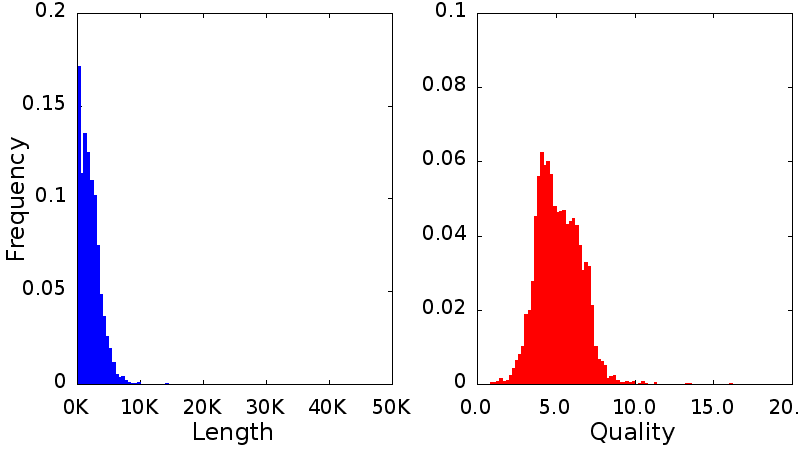
\includegraphics[width=.5\textwidth]{images/lambda_R6.png}
}
\subfloat[R7 (2014/09/16)\label{fig:r7}]{
  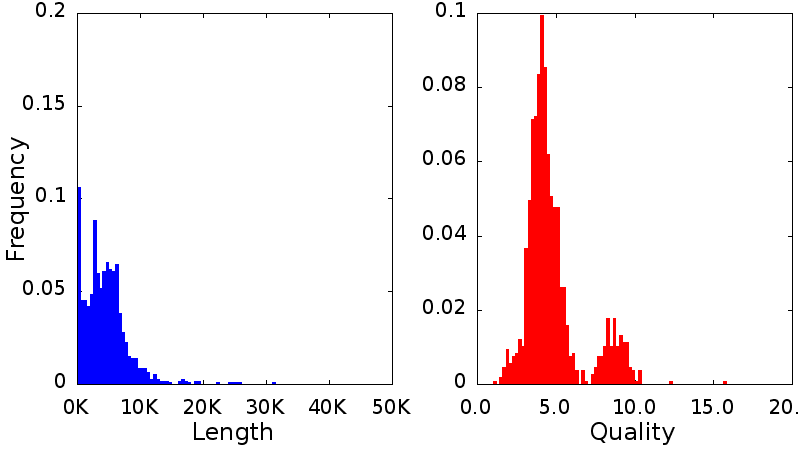
\includegraphics[width=.5\textwidth]{images/lambda_R7.png}
}

\subfloat[R9.4 (2017/01/18)\label{fig:r9.4}]{
  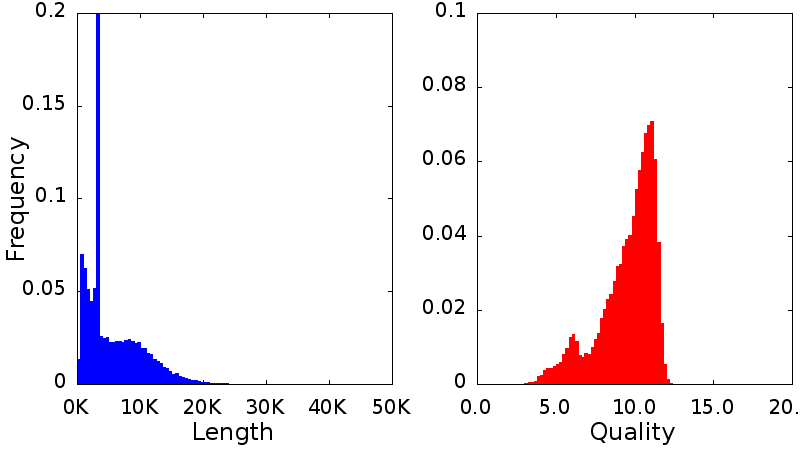
\includegraphics[width=.5\textwidth]{images/lambda_R9_4.png}
}
\subfloat[R9.5 (2018/09/12)\label{fig:r9.5}]{
  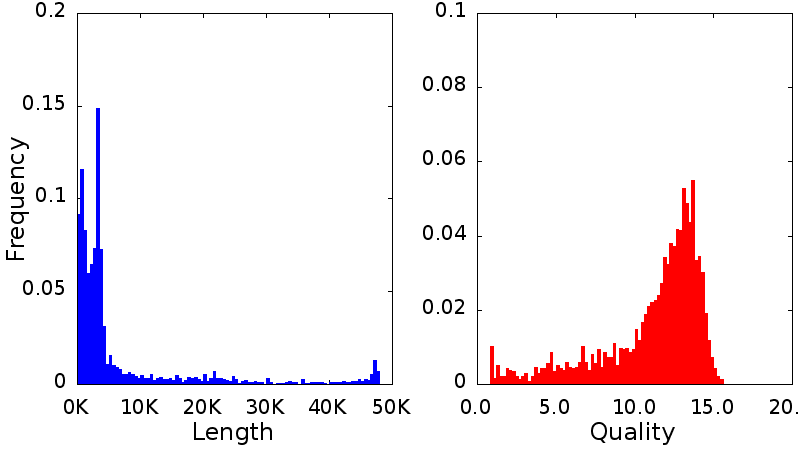
\includegraphics[width=.5\textwidth]{images/lambda_R9_5.png}
}

\caption[Statistics of nanopore burn-in experiments using different flow cell versions]{Statistics of nanopore reads using different flow cell versions (with the running date) on the lambda phage sample, shown in the order in which they were released. For each flow cell, the blue normalized histogram is for read length and red one is for quality (Phred score).}
\label{F:nnp_stats}
\end{figure}

\subsubsection{Lambda burn-in experiments} 
Figure \ref{F:nnp_stats} shows statistics of our lambda experiments acquired by using progressively more update version of MinION flow cells. This type of practice is a standard control `burn-in' experiment recommended by ONT to help users familiarize themselves with the protocol, the equipment and the result long-read data. The sample is a virus named lambda phage with small genome size of $50$Kbp. All the test experiments were run for 6 hours, except R9.5 with a 1-hour run so the sequencing yields are not included in the comparison and the histogram frequencies are normalized by the number of reads for each attempt. Even though the `burn-in' experiment is not designed to exhaustively study the potential length of nanopore reads due to the limit genome size of the sample, it is easily to see from the figure a clear improvement of read length distribution by applying newer version of flow cells. The early-staged (2014-released) flow cells and chemistry in the kit produced fewer reads longer than $10$Kbp, as could be observed from Figure \ref{fig:r6} and \ref{fig:r7}. 
This remarked value has become the mean length of reads generated by R9.4 flow cell which can even possibly reach $20$Kbp in extreme cases. 
Using the newest available flow cell R9.5 - even for just a 1-hour run - produced many more longer reads, including the maximum possible $50$Kbp reads that cover the whole genome.  
Similarly, the fidelity of the long reads has improved with the 2016-released R9 flow cells. The average quality scores (in Phred scale) of the base-called sequences have advanced from $5.0$ ($P_{error} \approx 0.3$) in R6 and R7 to $10.0$ ($P_{error} \approx 0.1$) in R9.4 and $13.0$ ($P_{error} \approx 0.05$) in R9.5. 
To further enhance the quality, reads from two complementary strands can be sequenced and computationally merged to produce a single double-checked 2D or 1D$^2$ read.
% Accordingly, the latest R9.5 pores and new base-calling algorithm can help improving the quality of long reads to around 95\% accuracy for single-stranded (1D) and are even aiming at 99\% for 1D$^2$ reads.  %%LC comment - not sure relevant what there aim is, better to stick to what has been achieved
Even so, noises will inevitably remain in nanopore reads as the result of measurement noise at nano-scale, as compared to high-precision data generated by SGS when the average Phred score is usually 30 or more ($P_{error} \leq 0.001$).

\subsubsection{The first runs with bacteria data} 

\begin{table}[ht!]
\centering
\small
\caption[Sequence two \emph{K. pneumoniae} strains with the MinION]{Sequence two \emph{K. pneumoniae} strains with the MinION. Figures generated by \npreader{} GUI \cite{CaoGC2016}.} 
\label{tab:first}
 \begin{tabular}{lccl}
 \hline
 \toprule
 \textbf{Strain} & \textbf{Phred Quality Scores} &\textbf{ Read Length Distribution} & \textbf{Emp. errors} \\
 \hline
   BAA-2146 & & & Del: 9.5\% \\ 
   (NDM-1 strain)& \multirow{4}{*}{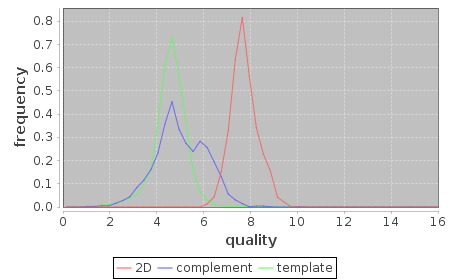
\includegraphics[width=0.33\textwidth]{images/qualR7.png}}    & \multirow{4}{*}{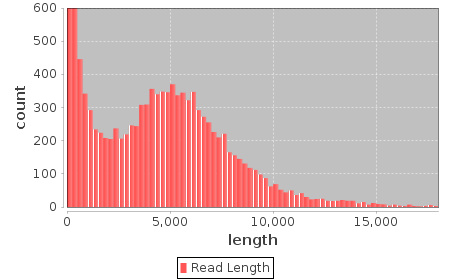
\includegraphics[width=0.33\textwidth]{images/lengthR7.png}} &  Ins: 6.3\% \\
    & & & Mis: 15.3\% \\    
   Chemistry R7& & &  Unaligned:  \\
   Sep 2014& & & \ \ \  13.3\% \\
   35-X Coverage& & & \\ \hline  
   
   13883 & & &  Del: 7.9\% \\   
   (type strain)& \multirow{4}{*}{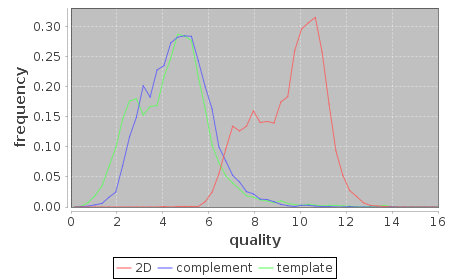
\includegraphics[width=0.33\textwidth]{images/qualR73.png}} & \multirow{4}{*}{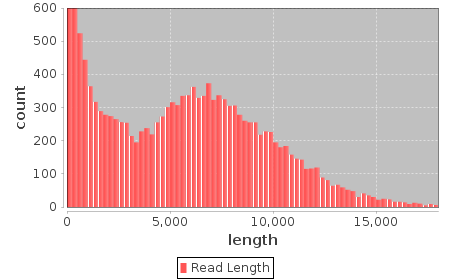
\includegraphics[width=0.33\textwidth]{images/lengthR73.png}} & Ins: 6.0\% \\
   & & & Mis: 12.9\% \\   
   Chemistry R7.3 & & & Unaligned:  \\   
   Dec 2014 & & & \ \ \ 11\%\\
   15-X coverage & & & \\ \hline
 \end{tabular} 
\end{table}

Amongst our first-hand experiments with real-life samples were the ones with \kp{} strains as shown in Table \ref{tab:first}. Flow cell version R7 and R7.3 with 2D sequencing protocol were used for the runs resulting in 35-fold coverage of long-read data for NDM-1 strain and 15-fold coverage for the type strain. From the quality histograms, the red lines represent 2D reads' scores which are clearly better than the ones in 1D reads (green and blue for template and complement sequences respectively). The length distribution shows that MinION sequencing returned significant reads with length around $5K$ for the first sample and $7K$ for the latter. The statistics on the far right of the table show error rate in term of indels, mismatches and hit rate from alignments with reference data. Overall, chemistry R7.3 is more up-to-date than R7 and as expected, gave slightly better results. 
As a next step, there came a mission to assembly those reads, together with available Illumina data of corresponding samples, in an attempt to have complete genome reconstructions for these two \kp{} strains. This task was important at the time as it would depict bigger picture about interactions between genetic elements in the whole genome and help to comprehend the biological pathways supporting this superbug's mechanisms.   

\subsection{Data analysis: challenges and solutions in working with nanopore data}
The introduction of long, error-prone nanopore reads has motivated novel developments in bioinformatics, as many existing approaches had been optimized for high-quality short read data.
A class of efforts was made to carry out an initial error-correction step before using the dataset~\cite{GoodwinGE2015,MadouiEC2015}. 
This process usually require either another reference of high quality SGS reads or a large amount of long reads for self corrections.
The majority of algorithms following this approach uses alignment-based correction which is normally costly in term of computation.

Another attempt to reduce the error rate from base-called sequences is to utilize the signal-level information. Nanopolish is designed for such task. The underlying technique is to train a hidden Markov model that measures the probability of observing a certain chain of events given a particular DNA sequence. This method has been used for polishing a draft assembly using an abundance of long-read data~\cite{LomanQS2015} and has been extended to detect methylation~\cite{Simpson2017methylation}. Nevertheless, this approach is computational expensive and usually requires parallelization which is supported in its modules.

Pairwise sequence alignment is a critical operation for many genomic analyses in general and  comparative studies in particular. To adapt to the specific error characteristics of nanopore sequencing data, a number of approaches has been introduced on top of the legacy alignment methods used for short-read SGS data. 
The ubiquitous practice is still based on the previous seeds-and-extend dynamic programming technique with modifications in term of seed finding, gap extension and chaining algorithms. In addition, there would be justified settings to relax the matching criteria thus allowing more error tolerance and lengthen the alignments. As the results, early long-read alignment tools have been developed or calibrated for PacBio SMRT data, including but not limited to BLASR~\cite{ChaissonT2012}, LASTZ~\cite{Harris2007lastz}, LAST~\cite{KiełbasaWSH2011}, BWA-MEM~\cite{Li2013} and DAligner~\cite{Meyer2014daligner}.
Recently, several other tools has been designed specifically for comparing long-read data such as GraphMap~\cite{Sovic2016graphmap} and especially $\mathtt{minimap}$~\cite{Li2016} (now \minimap{}) which significantly reduce the running time while maintaining comparative accuracy at the same time.
These available solutions have been widely applied in a flexible ways for different analysis purposes when it comes to long reads with high error rate.

The problem of aligning raw long reads stems from the error profile per base in the targeting sequences, especially indels, that would introduce combinatorial explosion using traditional approaches. The common practice to tackle this problem is to apply \emph{hashing} techniques to reduce the dimensional of the data. A hash function maps a particular string to an index value so that it can be accessed directly without (or minimized) collision. By using these functions, a DNA sequences can be represented by a small set of fingerprints, known as sketch, that will be shared between similar but not necessary exact strings.
The prominent sketch types that has been used for nanopore data includes MinHash~\cite{Ondov2016mash,BerlinKC2015}, minimizer~\cite{Li2016}, HyperLogLog (\emph{Dashing: Fast and Accurate Genomic Distances with HyperLogLog} 
Daniel N Baker, Benjamin Langmead.
\textbf{bioRxiv} 501726; doi: \url{https://doi.org/10.1101/501726}
).

For the multiple sequence alignment (MSA) problem, the partial order alignment (POA) graph data structure has been proposed to cope with errors in long reads~\cite{Lee2002multiple,Lee2003generating,Grasso2004combining}. By applying this method, the authors proved the integrity of information compared to other MSA format and developed POA as an efficient tool for large alignment and consensus calling problem. The latter was then adopted in Racon~\cite{Vaser2017racon}, a commonly used consensus module for long uncorrected reads.

Genome assembly is another major challenge in bioinformatics when the traditional approaches for SGS data cannot be applied directly to TGS data.
To better understand the situations and come-up solutions, the general principle of genome assembly and methods for SGS data will be addressed in the next section.
Approaches to genome assembly which utilize nanopore reads will come later on top of this foundation knowledge. 

%%%%%%%%%%%%%%%%%%%%%%%%%%%%%%%%%%%%%%%%%%%%%%%%%%%%%%%%%%%%%%%%%%%%%%%%%%%%%%%%%%%
%%%%%%%%%%%%%%%%%%%%%%%%%%%%%%%%%%%%%%%%%%%%%%%%%%%%%%%%%%%%%%%%%%%%%%%%%%%%%%%%%%%%%
%%%%%%%%%%%%%%%%%%%%%%%%%%%%%%%%%%%%%%%%%%%%%%%%%%%%%%%%%%%%%%%%%%%%%%%%%%%%%%%%%%%%%
\section{Genome assembly}\label{sec:gass}
\subsection{Definition}
\begin{figure}[ht!]
\centering
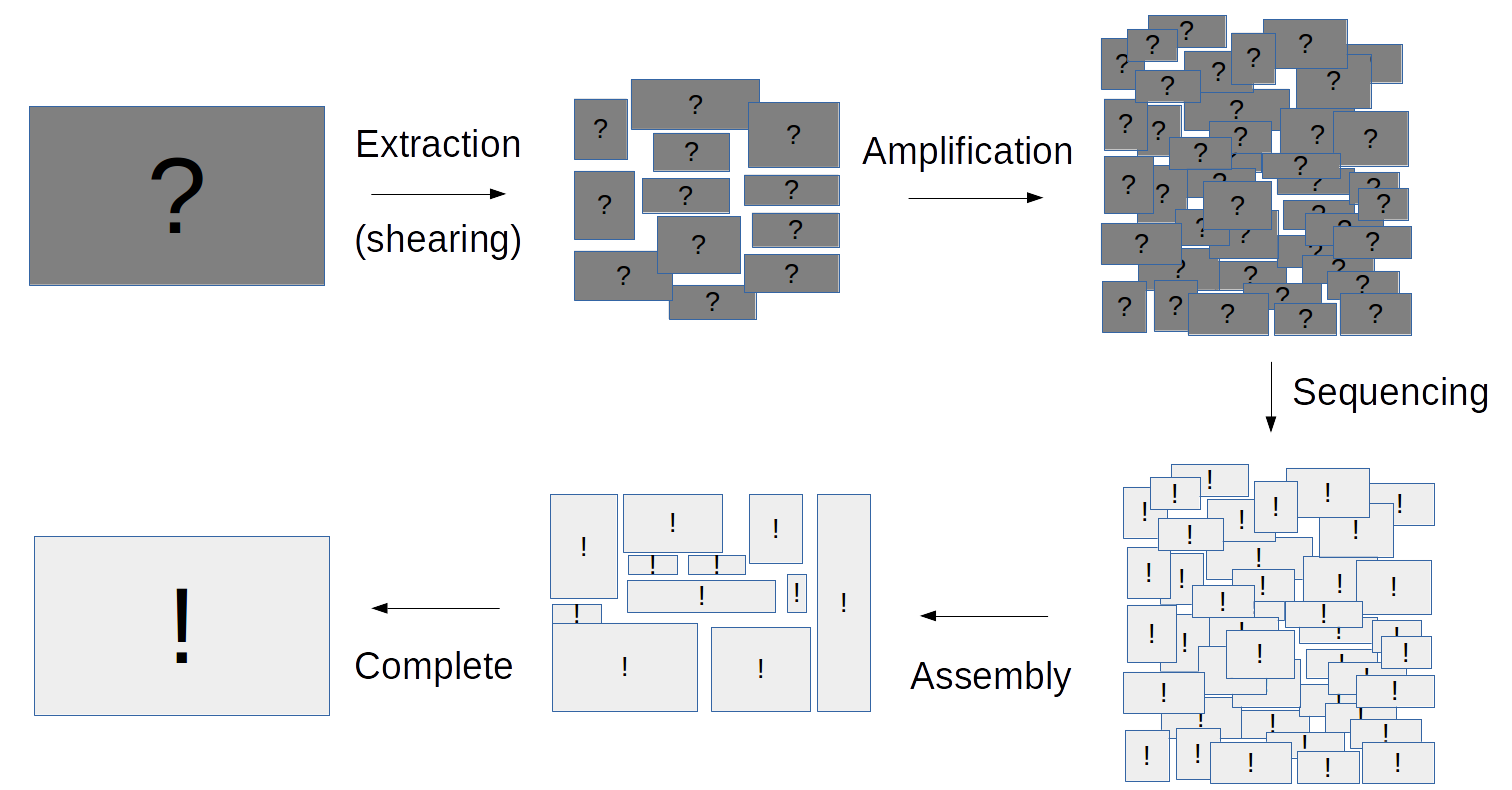
\includegraphics[width=.9\textwidth]{images/genome_decoding.png}
\caption{Basic framework for genome decoding process.} 
\label{Fig:decoding}
\end{figure}

Despite the huge improvements of sequencing technology, there still exist the common limitation that in most cases, it is impossible to sequence directly the whole length of a genome. As shown in Figure~\ref{Fig:decoding}, the actual practice is to break the whole genome into smaller pieces that could be efficiently read by an appropriate instrument. 
Before sequencing, the extracted DNA sample is normally sheared , \EG{} by restriction enzymes, into short fragments before being subjected to a cloning step, usually Polymerase Chain Reaction or PCR, that generates a large amount of copies for DNA molecules~\cite{Garibyan2013research}. The rationale is to have enough coverage to compensate the stochastic errors which are inevitable during library preparation and sequencing process. 
Those amplified pieces are then glued back together in a process called \emph{assembly} to have a draft genome prior to applications of additional post-processing steps for the final complete reconstruction.  
These include but not limit to scaffolding, gaps filling, genome polishing and circularizing if applicable.
The last two tasks are carried out with computational tools and in many cases, being referred together as in one whole common mission known as \emph{genome assembly}. 

Among all the steps involved in WGS, genome assembly undoubtedly plays a critical role in DNA sequencing since it determines how complete and accurate the picture of whole genome is. 



\subsection{General working principle for genome assembly}

\begin{figure}[ht!]
\centering
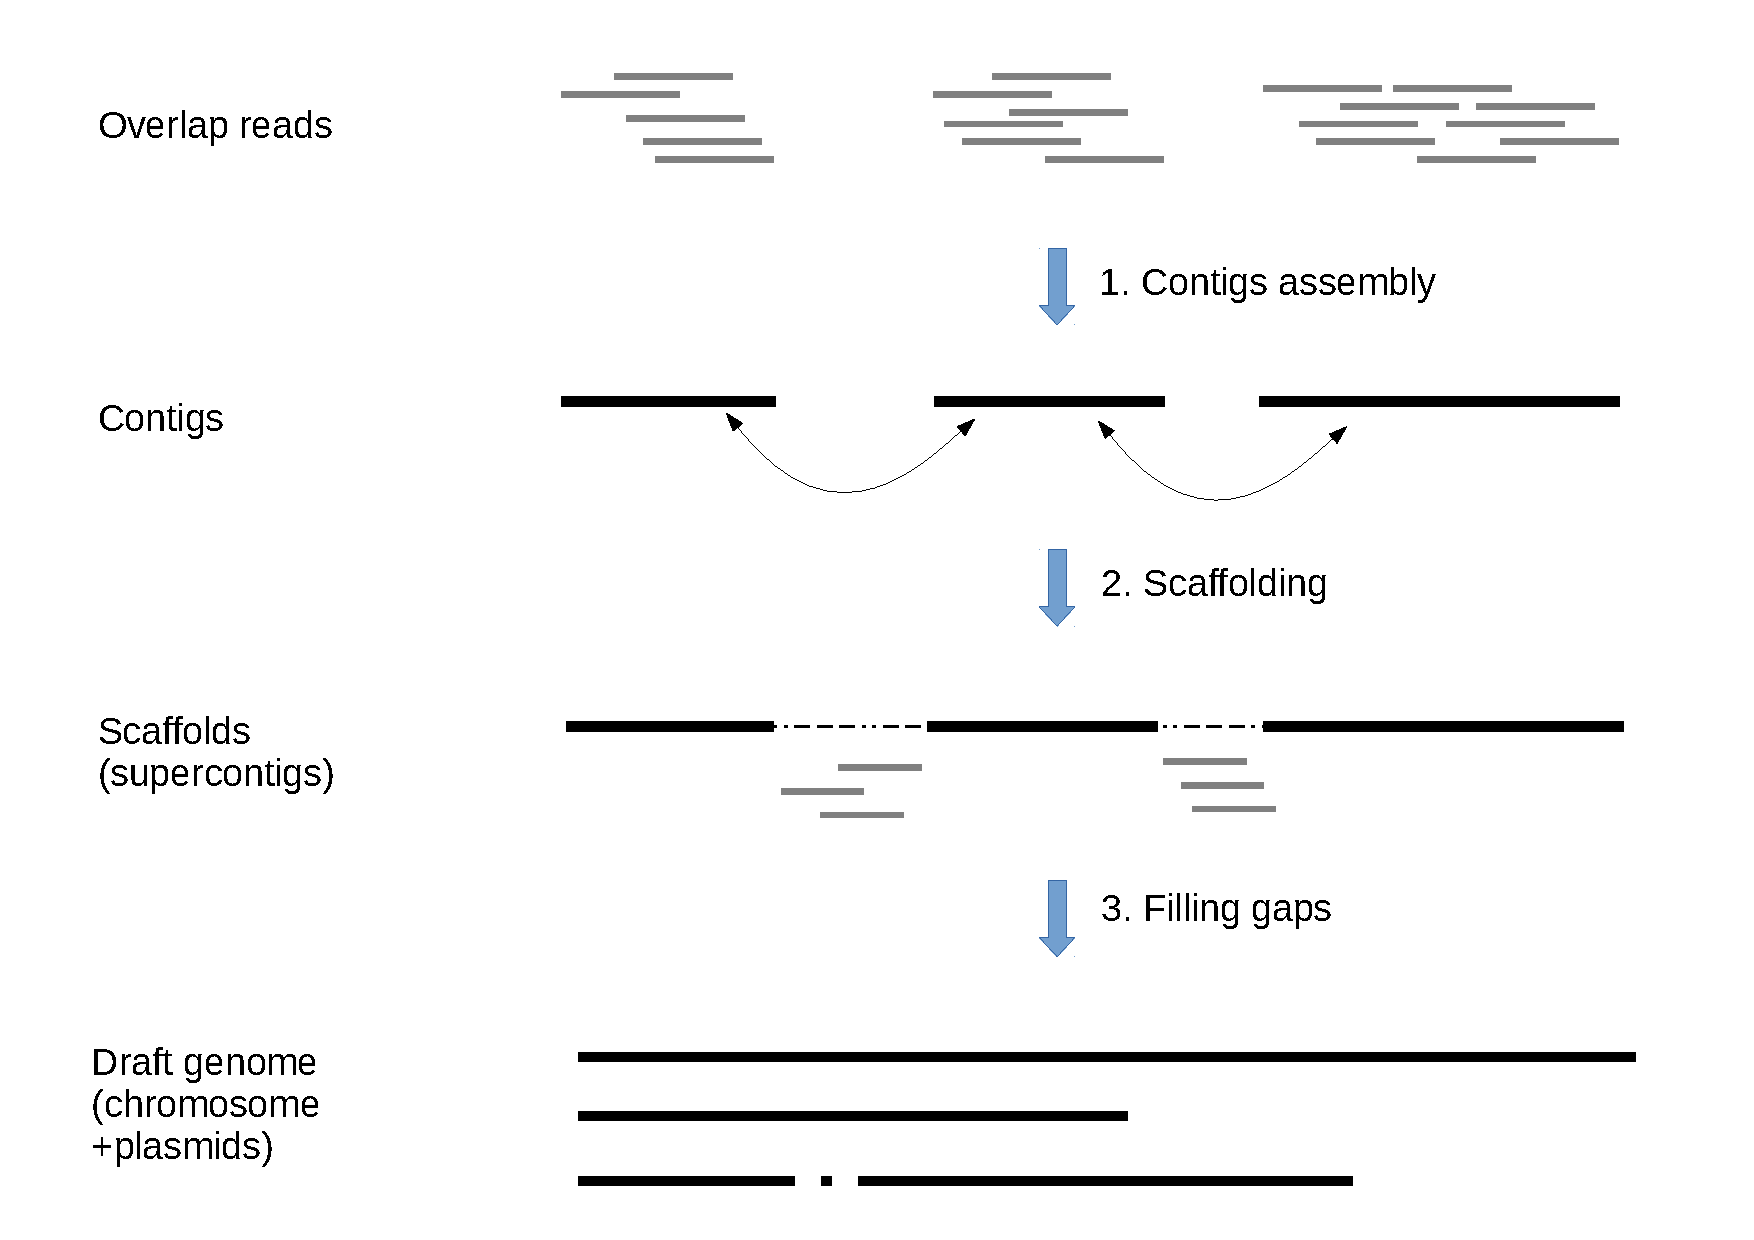
\includegraphics[width=.9\textwidth]{images/sassembly.pdf}
\caption{General assembly pipeline for short-read data.}
\label{Fig:assembly}
\end{figure}

A typical short-read assembly workflow would include three stages as shown in Figure \ref{Fig:assembly}. Firstly, the overlapping reads are merged together making up longer, un-gapped sequences named as contigs. Usually this is the most challenging and time-consuming part of the whole process, especially when the the number of reads is extremely large. The next step is to connect the fragmented contigs further by taking advantage of linking information from large insert reads \EG{} paired-end or mate pair data. The results are structures known as super-contigs or scaffolds that may contain estimated gaps. The final stage is to carefully fill those spaces by appropriate independent reads. The scaffolding and gap filling steps can be invoked repeatedly until no more improvement can be made \cite{Tsai2010improving,Boetzer2012toward,Paulino2015sealer}. The final result is a draft genome which consists of the longest possible stretch of sequences that can be induced from the data and algorithm. Unfortunately, it is common to not having the complete genome after this due to the repetitive nature of the DNA sequences. In fact, the fraction of fully completed genomes available in public databases such as GenBank (National Center for Biotechnology Information or NCBI) or European Bioinformatics Institute (EMBL-EBI), is comparatively small. Most of the assemblies are only near-completed, marked as contig- or scaffold-level, meaning that they are still fragmented and/or gap-bearing and require more work and data to become finished. 

\subsection{Overview of assembly algorithms for SGS data}
 
The demand for robust assemblers became overly compelling when high-throughput sequencing platforms were employed and started generating massive amount of data in the age of SGS.
The abundance of randomly distributed short reads from SGS platforms had motivated substantial research in bioinformatics toward solving the genome assembly problem in an efficient way\cite{Liu2012}. 
In general, approaches can be divided into two groups: greedy and graph-based approaches which are reviewed by \cite{MillerKS2010,LiZ2012}.
Greedy algorithms \cite{Sutton1995,Green1999,Huang1999} simply assemble all the reads by iteratively joining the two with largest overlap to form the shortest common string, or \emph{supersequence}.
It is noteworthy that greedy approaches implicitly use an overlapping graph as the data structure for this purpose. 
Clearly, the obtained result will be locally optimal and not necessarily the full solution to the problem. However, tools of this category usually produce a relatively good approximation \cite{Simpson2015}. 

The graph-based methods utilize data structure of vertices and edges to represent the whole set of reads and all of their potential linkage properties.
By traversing through the graph, one can define an assembly as an ordering reads and by searching for the best paths, find candidates for the optimal solution.
There are two types of graph in common use, namely Overlap--Layout--Consensus (OLC) \cite{Staden1979} and de Bruijin graph (DBG) \cite{Idury1995,PevznerTW2001}. 

\paragraph{Overlap--Layout--Consensus} The classical OLC algorithms follow the following three steps: overlap finding, layout forming and consensus calling. Throughout the process, an \emph{overlapping} graph is created which has vertices as reads and edges are represented by overlapped pairs of reads which have been detected based on alignments in the first step. A traversal algorithm is then applied to find the paths of ordered and oriented vertices, also known as the \emph{layout}. The consensus sequences are called and output based on the layout detected.
Among all the steps, finding overlap between all pairs of reads is the most computationally intensive. Although indexing techniques, such as FM index \cite{FerraginaM2005}, have been applied to reduce the time \cite{Ning2001}, the first step still remains the major bottleneck in the whole process, especially with the burst of short read data yield introduced by recent Illumina platforms.
In that circumstance, the DBG has come to be used as an efficient data structure to deal with this abundance of data. 

\paragraph{De Bruijin Graph} To construct the graph, reads are broken into consecutive \emph{k-mers} (words of length $k$) for the set of vertices, whilst edges show adjacencies between \emph{k-mers} with $k-1$ overlap. The data structure is actually storing fixed-length words and their linkages, making its memory requirement dependent only on the genome size but not data size. The graph is then targeted to errors removal based on \emph{k-mers} spectrum, as well as trimming and simplification in which non-branched paths are merged together.
At this point, the assembly problem can be reformulated as finding an Eulerian path which defined as a walk visiting each all edges on the simplified graph exactly once. 
The complexity of this algorithm is dependent on properties of the \emph{k-mers} rather than the number of reads. With a smaller $k$, the more details of overlaps emerge in the graph, but the trade-offs would be a bigger search space due to increasing number of nodes and edges. The reason for additional connections comes from the raise of repetitive elements not covered by the word length, resulting in more branches to traverse through the graph.  
Currently, there are several prominent DBG-based assemblers such as Velvet \cite{Zerbino2008}, SPAdes \cite{BankevichNA2012} and ABySS \cite{Simpson2009}. All of these work efficiently on Illumina HiSeq or MiSeq output with reasonable resources and running time requirements. In term of small genomes, such as bacterial genomes, which are the focus of this thesis, SPAdes is reported to be the most suitable tool amongst the three \cite{Magoc2013}.

\begin{figure}[ht!]
\centering
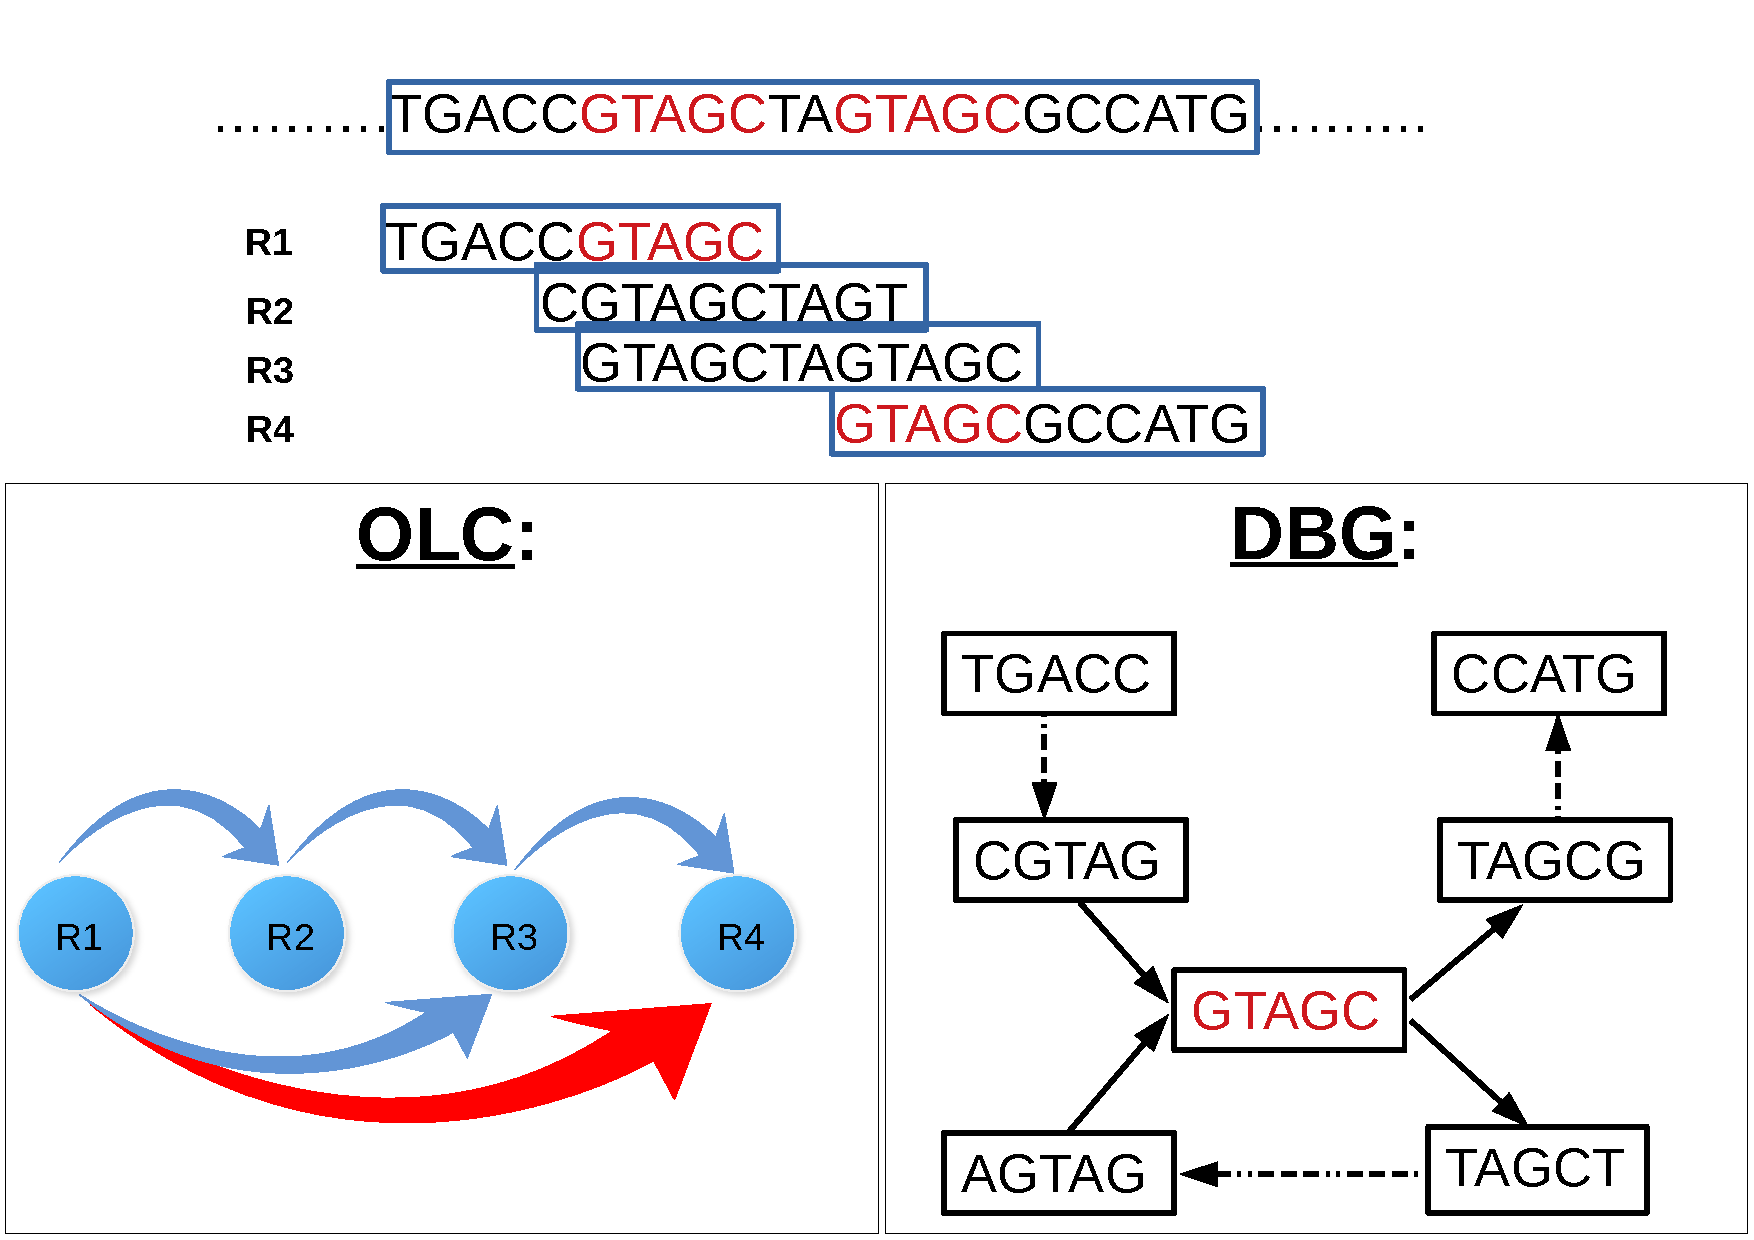
\includegraphics[width=.8\textwidth]{images/olcdbg.pdf}
\caption[Example about building OLC and DBG graph from a string]{A simple example about building OLC and DBG graph from a string with repeat (highlighted in red). The repeat introduces ambiguous alignment resulting in a redundant link (highlighted) in the overlap graph. It also de-linearizes the DBG graph by introducing a branched node corresponding to the repetitive \emph{k-mer}.}
\label{F:olcdbg}
\end{figure}

Figure \ref{F:olcdbg} gives an illustration of the graph construction by applying either the OLC or DBG approach.
A random string containing repetitive elements is given as the reference, from which reads are sampled as output from a short-read sequencer working on this imaginary genome. 
Using the OLC approach, a graph is built with reads as vertices and edges reflecting overlapping properties between pairs of them. Each time a new read is generated, there is one more vertex being added to the graph and by pairwise alignments to every other vertices, new edges can be added properly. To reduce size of the layout graph as the dataset is growing, the algorithm usually tries to remove contained nodes and redundant edges, \EG{} $R2$ in the example since it is covered by $R1$ and $R3$ together. The repetitive elements cause additional faulty alignment, \EG{} the red link from $R1$ to $R4$, making it more complicated to traverse the graph in the correct sequence.

On the other hand, DBG approach first breaks reads into set of consecutive \emph{k-mer}s ($k=5$ in this case).
Unlike OLC, no pairwise alignments need to be explicitly carried out. 
As the consequence, the DBG graph is more efficient in term of construction, however, would be more challenging to solve compared to the reduced OLC graph. The reason stems from the fact that the integrity of reads are usually lost after being broken into smaller pieces as $k$ must be strictly less than the read length. 
At the same time, the repeat nature of original sequence would split the OLC nodes into extra branches compared to DBG counterparts, making it more fragmented and difficult to traverse.
It is worth to mention the importance of parameter $k$ for the DBG performance. 
As aforementioned, $k$ should be chosen as large as possible to restraint the loss of information and the complexity of the resulting graph. However the graph would suffer the risk of disjointed components, or dead-ends, if $k-mers$ becomes too long so that one word would less likely overlap with another by $k-1$.
From the example, we chose $k=5$ as the best option since the DBG with $k=6$ would fail to represent the overlap between R3 and R4.

As mentioned earlier, genome assembly from SGS data usually suffers from the presence of repeats, leading to generation of highly fragmented draft genomes (also known as pre-assemblies). This limits identification of structural variation, or identification of the configuration and location   of mobile genetic elements.
One theoretical solution is to have reads that exceed the `golden threshold' of $7000$ nucleotides to span over the majority of repeats in prokaryotes \cite{KorenP2015}, thus able to connect fragmented contigs and render continuous assemblies out of them.
In fact resolving repeats has remained a bottle-neck until the recent emergence of the so-called Third Generation Sequencing technologies with the introduction of two instruments PacBio RS and Oxford Nanopore MinION that were specially designed for long-read sequencing. Thanks to these sequencers, DNA molecules with continuous length of up to tens of kilo base-pairs or even more could be sequenced in full.
As a result, long-read data have been widely exploited to finish genomes \cite{BashirKR2013,KarlssonLS2015} or identify mobile genetic elements of interest \cite{HudsonBM2014,AshtonND2015}, despite having a higher base-calling error rate.
A class of assemblers using these new instrument's output has been developed, which I will describe in the following section.
%\vfill
%%%%%%%%%%%%%%%%%%%%%%%%%%%%%%%%%%%%%%%%%%%%%%%%%%%%%%%%%%%%%%%%%%%%%%%%%%%%%%%%%%%
%%%%%%%%%%%%%%%%%%%%%%%%%%%%%%%%%%%%%%%%%%%%%%%%%%%%%%%%%%%%%%%%%%%%%%%%%%%%%%%%%%%
\section{Genome assembly with long read data}
Nanopore data can be used on its own for \emph{de novo} genome assembly, or in conjunction with high quality SGS data in a process called hybrid assembly. 
Both approaches have their own pros and cons and should be considered in reference to available dataset and the ultimate purposes of using the final assembly.
\subsection{Long-read only assemblers}
Non-hybrid assembly tools, as stated above, follow either OLC and/or an adjusted DBG approach, described below. Accordingly, most of current OLC algorithms rely on a hierarchical approach~\cite{Jayakumar2017compare}. From this perspective, seeds are first chosen top-down as a subset of longest reads that must have good base-called quality and not contain each others. The remaining reads of shorter length are then aligned to the seeds for error-correction before invoking assembly and post-processing as usual.

Hierarchical Genome Assembly Process (HGAP)~\cite{ChinAM2013} was one of the first hierarchical OLC tool available for PacBio data but a more well-known assembler in this category is \emph{Canu}, a renovated version of \emph{Celera Assembler}~\cite{MyersSD2000} that was designed to work in particular with noisy long sequences. Canu employs a typical OLC approach with an adaptive overlapping strategy and sparse assembly graph construction to be able to build a correct overlap graph out of error-prone data~\cite{Koren2017canu}. Canu is able to generate decent final assembly for large eukaryotic genomes but usually requires a lengthy running time.
FALCON~\cite{Chin2016facon} is another assembler applicable to big genomes, more than that, its string graph is designed to be diploid-aware.
Another efficient OLC implementation is to apply a fast overlap finding algorithm first for the assembly skeleton, then use another consensus calling or polishing tool on the draft assembly to improve the quality. This idea has been integrated in SMARTdenovo (\url{https://github.com/ruanjue/smartdenovo}) or in a pipeline that combines 2 separately developed modules: \emph{miniasm}~\cite{Li2016} as the rapid draft constructor and \emph{Racon}~\cite{Vaser2017racon} as the consensus caller. 
%%LC comment - is this a good time to discuss minhash and other hashing approaches, like hyperloglog


Regarding to other class, \emph{Flye}~\cite{Lin2016abruijin,Kolmogorov2019Flye}  and \emph{wtdbg} (\url{https://github.com/ruanjue/wtdbg2}) are two representatives of long-read assemblers that used adaptive versions of \emph{de Bruijin} graph.
The first method introduces the definition of ABruijin graphs that only take a subset of ``solid strings'' instead of all fixed length words decomposed from reads. The solid strings are chosen based on the \emph{k-mer} spectrum from which their fidelity are examined.
Unlike the traditional DBG methods, a fast dynamic programming algorithm is used to evaluate the overlaps of various lengths between read pairs based on their longest common subpaths. The draft assembly is constructed by adding vertices of those overlapped reads before undergoing a polishing step by aligning it to the original reads.
The tool wtdbg (now wtdbg2) on the other hand, builds a fuzzy de Bruijin graph for genome assembly. This graph is similar to the original DBG but allows mismatches and indels so that approximate \emph{k-mer}s can be collapsed into one node of the graph. Furthermore, the read paths are kept during decomposition and collapsing. After layout construction with the fuzzy DBG, a POA-like consensus step is invoked to generate the final assembly. 
The tool is reportedly able to quickly finish an assembly but consumes more memory than an original DBG approach due to the new graph structure. 

For exclusive long reads assembly, the quality of assembly is in general lesser than SGS counterparts, even after a polishing step. 
As the consequence, additional polishing steps with Illumina data is desired for higher accuracy in \EG{} for SNP callings projects.
Another approach is to utilize the erroneous long reads as the linker to connect the incomplete SGS assemblies~\cite{DeshpandeFP2013,BoetzerP2014}. Assemblers from this class usually require less long read coverage. Moreover, bridging operations are much less resource-consuming than aforementioned approaches.  I expand on these hybrid assemblers in the next section. 

\subsection{Hybrid assemblers}

Hybrid assembly using long reads is an economical and efficient approach to retrieve more complete genomes from the drafts since it requires less runs of the currently expensive third-generation sequencing. 
One of the first algorithms that takes advantage of long reads for hybrid assembly is Cerulean~\cite{DeshpandeFP2013}. By aligning the contig sequences from short read assembly to the long reads, it tries to build a \emph{skeleton graph} of long contigs connected together as the backbone and later accompany smaller contigs iteratively to the backbone to improve the assembly quality. This tool provides an efficient way of finishing the draft genomes in the sense of running time and memory usage.
Likewise, in term of assembling with long-read data, SSPACE-LongRead~\cite{BoetzerP2014} stands out as a widely-used software for this particular task. 
Briefly, the method relies on the BLASR~\cite{ChaissonT2012} alignments between long reads and the pre-assemblies which are normally contigs resulted from short-read assemblers.
Based on the linkages from the best alignments, a placement of these contigs into super-scaffolds is established. 
The scaffolds will undergone a post-processing step of final linearization and circularization before being used as the assembly output.
This approach provided a cost-effective reconstruction of bacterial genomes by using two libraries: one Illumina MiSeq or Roche-454 paired-end reads and one 50-folds long reads data from PacBio.
Although long reads from other sources, such as MinION, can also be used by these methods~\cite{Karlsson2015}, it usually requires extra works on parameter calibration.

In addition, another scaffolding algorithm, LINKS~\cite{WarrenYV2015}, uses a \emph{k-mer} approach to make use of long reads properties rather than an aligner to connect the draft genomes. This method  succeeded in improving the contiguity of ABySS genome
assemblies and could adapt to a certain scale of eukaryotic genome. However, the performance highly depends on the data quality so that for early-staged chemistry of Nanopore sequencing, only 2D reads screening and/or application of error-correction utilities are recommended beforehand.
In ligth of that, beside several dedicated genome scaffolding tools for MinION data as above, users can always utilize the traditional approach of using error-free short reads to correct the nanopore reads at base level. After that, the corrected long reads can be assembled by a conventional OLC algorithm in the next step. Nanocorr~\cite{GoodwinGE2015} and NaS~\cite{MadouiEC2015} are two representatives for this approach. Normally, these assemblers could provide assemblies of high quality per base but with much more expensive computations in exchange. 

Finally, another appropriate software for this purpose is Unicycler~\cite{Wick2017unicycler} which has been developed as the state-of-the-art. This application is in fact a set of tools including a combination of short-read assembly optimization, long-read only assembly, hybrid assembly, consensus calling and other post-processing steps for microbial genome assembly. It is designed to work with either short-read or long-read data but focuses on the hybrid algorithm that take advantage of both type of datasets. 
Its hybrid assembly module works in a likewise non-interactive (batch) mode on the whole bulk of input data, traverses the input assembly graph and returns a exhaustively polished assembly as the result. 
This method has been proved to generate high quality, very close-to-complete genome assemblies thanks to exhaustive computational steps but the running time, as a trade-off, is relatively long and is only efficient for microbial genomes. 
More details about this method will be provided later in Chapter~\ref{ch:npgraph} as a relevant content.
%%%%%%%%%%%%%%%%%%%%%%%%%%%%%%%%%%%%%%%%%%%%%%%%%%%%%%%%%%%%%%%%%%%%%%%%%%%%%%%%%%%
%%%%%%%%%%%%%%%%%%%%%%%%%%%%%%%%%%%%%%%%%%%%%%%%%%%%%%%%%%%%%%%%%%%%%%%%%%%%%%%%%%%
%%%%%%%%%%%%%%%%%%%%%%%%%%%%%%%%%%%%%%%%%%%%%%%%%%%%%%%%%%%%%%%%%%%%%%%%%%%%%%%%%%%
\section{Real-time analysis}
\subsection{Definition}
In circumstances of this thesis, the adjective ``real-time'' indicates  a high level of responsiveness of an analysis system in updating its environment status corresponding to inputs fed into the system~\cite{Phillips1966programming}.
The time gap from getting new input to the point of status being updated, or \emph{deadlines}~\cite{Ben2006principles}, is not necessary to be as close to zero as possible (immediate), but in reality a positive value limited by a reasonable upper-bound (nearly immediate).
The upper-bound is normally defined based on human temporal sensation \EG{} within minutes.

Briefly, real-time data analysis is the operation applied on the data in a prompt time interval to provide near-instantaneous output.
In contrast, a data processing system is known to work in ``batch mode'' if it collects all the input data before any any operation is applied. 
The result obtained from a batch analysis on the bulk of data is final and static, meaning it cannot be updated using another batch of data without rerunning the whole process.
Real-time applications usually involve a specific communications method namely \emph{data stream}. Streaming data is characterized by its continuously migration from a \emph{source} to a \emph{sink}, which are normally the consecutive modules in a real-time pipeline.
To implement instant response programs is a challenging task but in return, grants certain amount of advantages over traditional batch counterparts~\cite{Croushore2011frontiers}. 
This will be discussed later throughout the content of this thesis.
\subsection{Real-time analysis for nanopore sequencing}
One of the novel aspects of ONT's sequencing platforms is that the sequence data of each molecule is written to disk as soon as it is generated (with up to 2000 molecules being sequenced in parallel, each molecule progressing through the pore at $450$bp per second).    This is unlike SGS sequencing-by-synthesis platforms, which sequence billions of short reads in parallel, with each cycle (contributing an extra base) taking several minutes, with the data being provided in batch at the end of a run.

For this task, the raw data of a read must be retrieved and analyzed while sequencing is still in progress. This offers the opportunity to obtain analysis results as soon as sufficient data are generated, upon which sequencing can be terminated or used for other experiments.
As the consequences, answers to the related genomic questions could be obtained \emph{in situ}, in an automated manner that saves considerable amount of time and resources compared to the conventional approaches.
Furthermore, streaming analysis can benefit from avoiding under- and over-sequencing which could result in either the generation of more sequence data than is required at greater cost, or a low quality assembly if insufficient data are generated. 

Several systems incorporating real-time feature of MinION data have been developed e.g. the cloud based platform Metrichor (Oxford Nanopore), work by Quick\etal{}~\cite{QuickAC2015} and MetaPORE~\cite{GreningerNF2015}, focusing on phylogenetic analysis of a sample. 
Importantly, it is worth noting the selective sequencing protocol, \IE{}``\emph{Read Until}'', which had been proposed and implemented~\cite{LooseMS2016} exclusively for nanopore sequencing, motivated by the idea that only DNA molecules of interest should be sequenced. In this proposal, the process could intervene the transition of DNA through the pore by reversing the pore bias to eject the one deemed as non-informative. To achieve this, an examination is carried out for each molecule by reading the real-time squiggle data from current changes caused by the transition and comparing this signal to a reference. This real-time feedback system would be important for target enrichment and background depletion sequencing \cite{Edwards2018real}. 

On the other hand, as a member one of the very first groups having access to MinION sequencing, I have been developing an in-house tool set to analyze the data for specific studies, focusing in streaming analysis on microbial genomics.  
The framework had been implemented with utilities ranging from initial analysis to handful of further identification processes such as species typing, strain typing and investigating antibiotic resistance profiles on microbes~\cite{CaoGE2016}. In such pipelines, \npreader{}~\cite{CaoGC2016} continuously scans the folder containing sequencing data in parallel with the MinION sequencing. It picks up base-called sequences as soon as they are generated, and a stream of reads is created to feed the  appropriate pipeline for further identification analyses. 
Different modules of a workflow can communicate to each other via the network sockets or inter-process redirection pipes provided by Unix-like operating systems.
In general, each module takes a stream of data of interest (\EG{} a read, an alignment) as input and carries out its task every time a given amount of data or waiting interval has passed. As a response, only relevant information is extracted to retain or forward to another module following the analysis. 
This data processing methodology can return results on-the-go and at the same time, only engages small memory footprint which is a clear benefit when working with large amounts of data, over long period of running experiment.  
Our tools are proved to be helpful in reducing the turn-around time for the clinical analysis and heading toward rapid diagnostic usage of MinION in real-life applications~\cite{Bialasiewicz2018rapid}.

However, there still exists a gap for a method that could scaffold and finish assemblies in a real-time fashion.  % as of MinION's output.
This has become the motivation for this thesis project which will focus on using nanopore data in the scaffolding and annotating feature of \npscarf{}, demultiplexing algorithm from \npbarcode{}, as well as assembly graph resolving in \npgraph{} - all working in real-time.

\section{Summary}
To sum up, for the time being, there are various DNA sequencing platforms available in the market, each of them embraces its own methodology and outputs different reads in term of length, accuracy, throughput and sequencing cost. Hence the choice for a sequencing method depends on the requirement from individual project and sometimes, users need to use several sequencers together on the same sample to obtain adequate data of interest. 
Amongst the sequencing options, ONT nanopore sequencing with MinION stands out as a remarkably portable and deployable long-read sequencer that offers real-time access to the sequencing output. The continuous upgrades of its flow cell and sequencing kits are indeed improving the quality and quantity of the long-read data, making this sequencing method a very welcomed additional player in the field.

MinION data has been shown to be a useful source of genomic data for various  studies thanks to its long-spanning and real-time accessible features. In the midst of those, genome assembly and structural annotation are amongst the most common applications since this technology can bypass the fragmentation caused by repetitive elements that are difficult to resolve using the short-read sequencing. At the same time, the on-time accessibility of the data opens up the opportunity to establish  analyses in real-time, thus offering interactive management on resources during sequencing process.
\section{Thesis aims}
Inspired by the unique functionality of nanopore sequencing technology, this thesis project aims to  develop real-time applications using MinION data, focusing on genome assembly pipelines for microbial isolates. The purpose is to have further complete assemblies, as much as possible, that would facilitate downstream annotations.

\paragraph{Goals setting} Initially, the project targets to implement a streaming pipeline to rapidly finish short-read assemblies using real-time MinION sequencing. 
It is aimed to join fragmented contigs with least input data as possible while at the same time, still able to producing high quality and complete sequences. 
The ability to run and to report completion status in real-time allows users to decide when to stop the sequencing prematurely thus open the possibility of saving time and cost for genome analyses.
In addition, hybrid assembly algorithm is expected to work on the assembly graph of the short-read assemblies to further improve the sensitivity and completeness of the final result. It would also provide users appropriate visualization for better interaction with the assembly pipeline in real-time.

On the other hand, it is desired to extend aforementioned pipeline for multiple samples at the same time, through a paralleling mechanism known as barcoded sequencing.
This technology is made available from ONT, via Barcoding kits, to allow pooling and sequencing of multiple libraries on the sample flow cell, which further enhances the versatility of the technology. The underlying mechanism is to ligate a unique oligonucleotide sequence, or \emph{barcode}, to the fragments of each DNA sample. Multiple samples can then be pooled together and sequenced in one flow cell. After that, the sequenced reads are demultiplexed into bins by examining the barcode portions on the reads. 
For this purpose, a streaming demultiplexer for barcode sequencing is developed.
The tool brings to MinION practitioners a flexible option to monitor a barcoded sequencing run as well as to integrate pooled sequencing into a streaming analysis pipeline.
Together with in-house software developments, their applications into real-life use cases are taken place. This would give better understanding about software performances as well as specifications on different datasets.

\paragraph{Contributions} 
This thesis resulted in several real-time processing modules that are able to assist genome assembly and annotation, including \npscarf{}~\cite{Cao2017scaffolding} \npbarcode{}\cite{Nguyen2017barcode} and \npgraph{}. 
All of these individual add-on modules were wrapped in a bigger framework that was specifically designed for nanopore data analysis, hosted in \url{https://github.com/mdcao/japsa}. 
The main contribution of this thesis regarding genome scaffolding and assembly can be found in a separate repository \url{https://github.com/hsnguyen/assembly} for the convenience of development and maintenance.

The source code of the whole project is made available and applied in numerous use cases internally as well as from community. Feedback from users and external data sources are treated with care to further improve the performance and functionality of the developing software. 

\paragraph{Restrictions}
The thesis mostly focuses on applications in microbial genomics as this is a clear use case for the applicability of real-time analysis particularly in diagnosis and identification of antibiotic resistance strains.  However, the methodologies developed in this thesis can be applied more broadly, and have been demonstrated on yeast genomes. Applications to metagenomics and eukaryotic genomes were attempted but not thoroughly studied thus not included in the scope of in this thesis.

Another limitation is that the developed assemblers are hybrid approaches, meaning an additional SGS run is required before using the tools. An exclusive long-read assembler is difficult to adapt to a real-time pipeline due to its intensive computation for the error-correction stage which usually requires bulk of data and heavy resources consumption.
\section{Thesis outline}
The main research chapters of this thesis are organized as follows.
\paragraph{Chapter 2}: 
This chapter presents the implementation of the very first pipeline for finishing genomes in real-time using MinION long reads and side applications through \npscarf{}.
\paragraph{Chapter 3}:
This chapter describes demultiplexing barcoded nanopore sequencing data with \npbarcode{} in real-time and its application. In addition, there is another use case of using different assembly strategies to finish four XDR \kp{} strains.
\paragraph{Chapter 4}: 
This chapter shows how to integrate assembly graph into the available pipeline from \npscarf{} to improve the assembly quality. This work results in \npgraph{} and relate applications.
\paragraph{Chapter 5}: 
This chapter introduces another computational analysis of MinION sequencing data for small circular genome assembly, such as for virus, bacterial plasmids. Data for two \emph{Caulimovirids} samples are shown to demonstrate the performance of proposed methods.